% ==================================================
% Appendix: Sensitivity of mean cosmics residual to area of region of interest %
% ==================================================
\chapter[Effect of area bin size on results]{Sensitivity of mean cosmics residual to area of region of interest}
\label{appendix-area_bin_size}

% --------------------------------------------------
\section{Effect of area}
% --------------------------------------------------

% DO I NEED TO EXPLAIN THIS IN MATH? I tried on June 3rd in my notes, it's complicated for such a simple thing.
% If this flies, you'll need to establish that reference frame == two fixed layers' frame as jargon in your thesis.
% Also need to establish x == perpendicular to wires; y == perpendicular to strips. ==> How do I do this consistently?
% May need to add 3100V reference if it's not already defined in your thesis.

The area of the region of interest in which to include tracks is primarily motivated by the misalignment model: the width of the area should be less than the scale on which the local offset is expected to change significantly. Changes in offset of order \SI{50}{\micro\meter} are important since this is the position resolution of the detector in the $\eta$ - coordinate. In a misalignment model with an offset and rotation, only the rotation changes the local offset with respect to the x-coordinate \footnote{The effect of rotation can be modeled by assuming the track position in the reference frame is related to the hit position by a passive rotation, where the angle of rotation is the relative angle of the layer of interest with respect to the reference frame. The local offset does change with respect to the track's y coordinate, but negligibly in the limit of small angles.}.  The distribution of cathode board rotations as calculated by the as-built model shows that the RMS of the rotation angle is \SI{200}{\micro\rangle} [https://indico.cern.ch/event/1035057/ PG. 18]; however the distribution has a long tail, so a typical rotation angle of \SI{1000}{\micro\rangle} was used here. A rotation of \SI{1000}{\micro\rangle} will cause a \SI{50}{\micro\meter} change in local offset over a change in x of $50 cm$. Therefore, the width of the region of interest should be less than $50 cm$.

Two other factors also inform the width of the region of interest. First, the width in x must be larger than the pitch of the wire groups to ensure the bin will have a sufficient number of tracks fall in it, since the hits' x-coordinates are discrete. Second, more tracks will be included in a larger area so more statistics will be available for the residual fit. For the bin widths above two wire groups, the statistics are sufficient. For each x-ray residual, the mean cosmics residual was calculated for a few different areas, and the difference in means plotted. \ref{fig:area_bin_size_mean_diff} shows an example for QL2.C.4. The width of the distribution is on the order of \SI{50}{\micro\meter}, showing that the calculation of the residual mean is relatively robust with respect to the area of the bin. However, \SI{50}{\micro\meter} is larger than the typical statistical uncertainty on the cosmic residual of means, which ranges from \SI{10}{\micro\meter} - \SI{40}{\micro\meter} depending on the tracking combination under study. Therefore, the cosmic residual means are assigned a flat uncertainty of \SI{50}{\micro\meter}. 

\begin{figure}
    \centering
    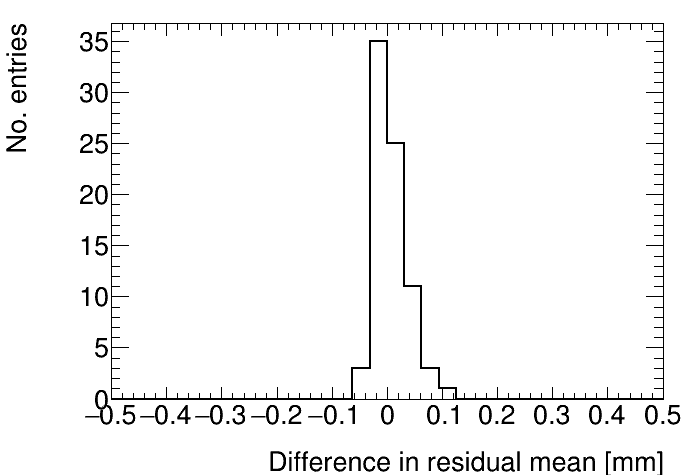
\includegraphics[width = \textwidth]{figures/compare_residual_fits_around_xrays_QL2C04_3100V_2021-05-20_100mm_width_bins_minus_QL2C04_3100V_2021-06-02_200mm_width_bins_means_difference.png}
    \caption{Difference in cosmics residual means around x-ray residuals for square bins of 100 mm width and 200 mm width for QL2.C.4.}
    \label{fig:area_bin_size_mean_diff}
\end{figure}